\section{Results}

\subsection{Course overview and development}

The workshop focused on the analysis and interpretation of neuroimaging data,
ranging from whole-brain functional magnetic resonance imaging (fMRI) to
single-cell microscopy. Instructors were distributed across three institutions,
and attendees were mostly graduate students and post-docs that had minimal
background in data analysis and image processing. The instructors took the
audience through detailed hands-on data analysis pipelines that harness open
source software for image processing  (\url{http://scikit-image.org/}
\cite{van2014scikit}, \url{http://nipy.org/dipy/}
\cite{Garyfallidis2014FrontNeuroinf}). They also introduced the participants to
machine learning techniques (e.g., deep learning methods using Caffe
\cite{jia2014caffe} and Tensorflow \cite{abadi2016tensorflow} as well an
introduction to scikit-learn \cite{Pedregosa2012-dm}).

All course materials were hosted via a shared online computing platform.
Students accessed this platform via web browsers on their own computers.
This made it possible to standardize the computing environment across both
students and instructors, and minimized the effort needed to get students
started with the material. In order to make course materials accessible in a
live, online computing environment, the following considerations were taken:

\begin{enumerate}

\item {\bf Software and computing environment}: The development of the course material was
performed in Docker containers. This ensured that all course materials could
run on any computing architecture that could host such a Docker image.
First, a Docker image
\cite{merkel2014docker} was created with the computational restrictions and
computing environment that would match what would be available on the cloud
platform we used. Instructors used a shared instance of this Docker
image while they developed sections of the tutorial independently. They used a
shared Github repository to host each section of the bootcamp, and pushed their
materials as separate folders in this repository. As new packages were needed in
order to cover particular topics, the base Docker image was updated with added
dependencies. As a result, by the end of course development there was a single
Docker image with all software tools needed to complete the course.

\item {\bf Data management}: Many bootcamp-style events require data to use in
the materials. For realistic research examples, the data can be cumbersome to
download and modify (for example, if many students attempt to download the
same file at once during class). This course covered a wide range of datasets
including publicly-available fMRI data
as well as images of cells collected from the human brain. Instructors used a
script that fetched this data from online repositories, and then stored it in
a common data folder on the user's computer. The Docker images were then
configured such that this script would be run as soon as a new image was
instantiated, ensuring that all data was pre-loaded onto the user's
filesystem upon launch. Because students had access to their
own computing environments, this data (and any modifications of it) persisted
over time and between computing sessions.

\item {\bf Environment distribution}: In the
day before the class, the course Docker image was deployed to several Virtual Machine (VM)
instances being run on the Jetstream cloud computing platform
\cite{Stewart2015Jetstream}, available through the Extreme Science and
Engineering Discovery Environment (XSEDE) \cite{Towns2014XSEDE}  (see section
\ref{sec:methods}). We chose this environment due to its presence on many
university campuses, though it is possible to use any cloud provider that
provides Kubernetes support such as Google Cloud, Microsoft Azure, or even
institutional hardware.

A single IP address was generated for each instance - one
for each student - and was sent out the morning of the event. Students only
needed to click on their respective IP address, and they were instantly taken to
a live Jupyter notebook contained within their XSEDE Jetstream computing
environment. This notebook had all course materials, as well as access to the
data, software packages, and live Python kernels that were needed to execute the
course materials. In addition, this environment persisted several days after the
class was finished in order to allow students to continue interacting with the
material, or to port their work onto their personal computers.

\end{enumerate}

\begin{figure}[h]
\centering
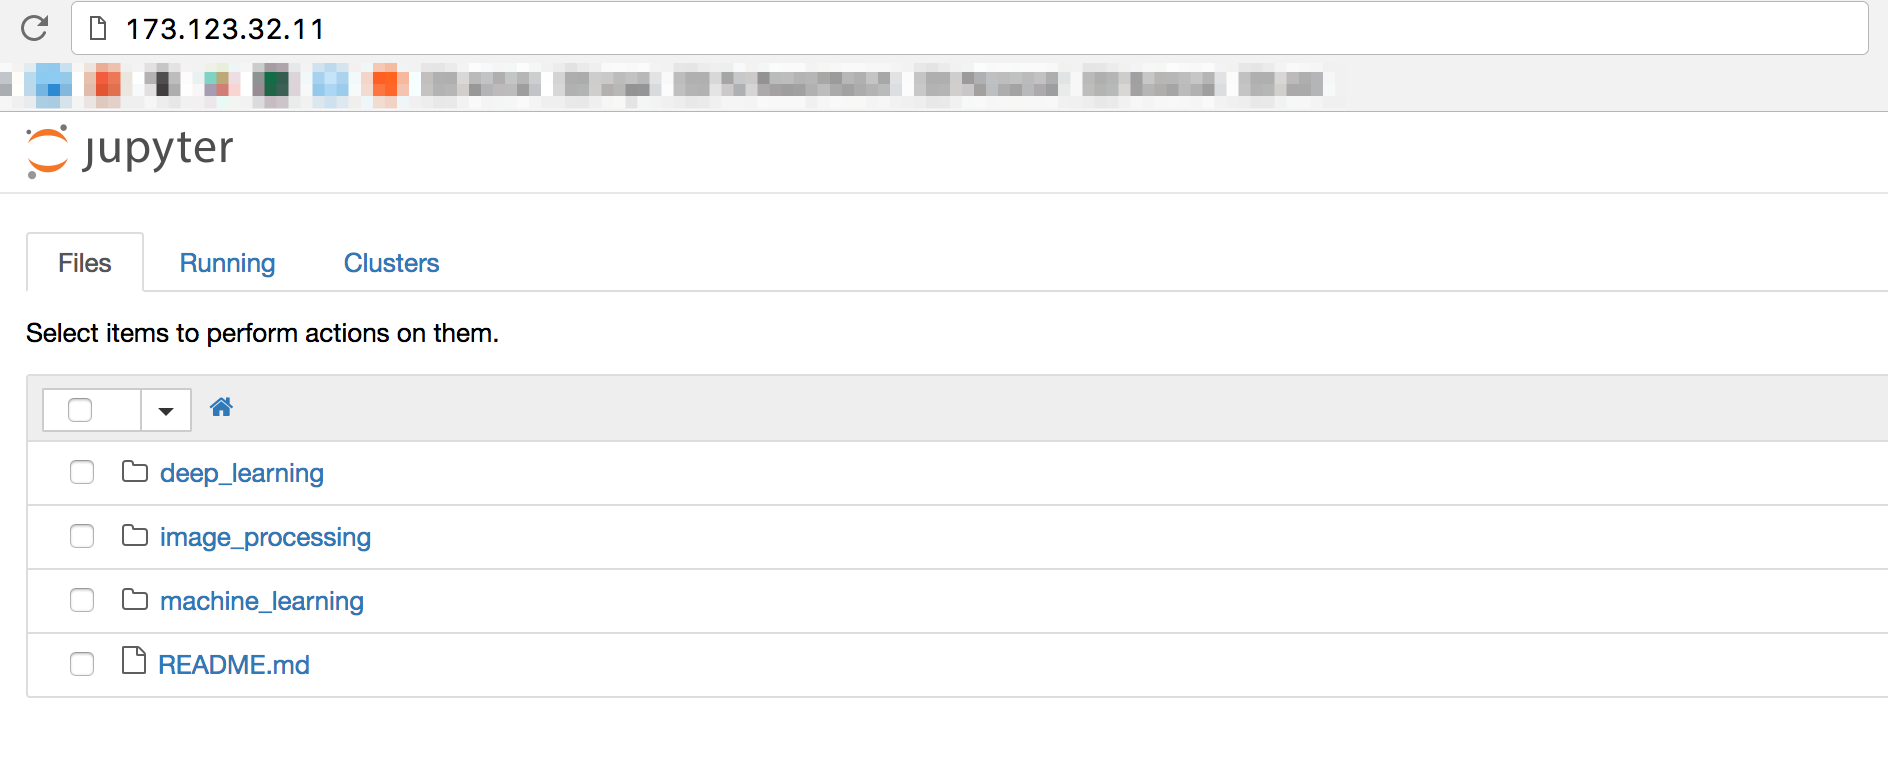
\includegraphics[width=0.5\textwidth]{sample_notebook.png}
\caption{Screenshot of a student notebook instance. Students were instructed to
         navigate to an IP address, and the resulting jupyter notebook was
         displayed with all course materials inside.}
\end{figure}

\subsection{Comparisons with a traditional bootcamp setup}

This section covers some of the main benefits and drawbacks of the cloud
computing approach towards bootcamp-style events. First we will cover primary
benefits of a 'traditional' bootcamp event (one in which participants are asked
to install the software on their own computers). Next we will discuss drawbacks
and how these are addressed by using cloud infrastructure. Finally we will
discuss new challenges that were introduced and how they might be addressed in
the future.

\subsubsection{Benefits of a traditional bootcamp approach}

The challenge of asking students to do all work on their own machines has one
primary benefit: they are operating in the computing environment that they
likely use on a daily basis. While it is common for frustrations to pop up
during installation and execution of course materials, these are also
quite common in every-day practice, and enable incidental learning
of the skills needed to know how to solve problems in general.
In addition, by doing all course computation on
their own computer, there is no need to adapt to a completely new computing
approach (beyond learning about new packages, languages, etc). Finally, after
the course is over there is no need to migrate course materials to new hardware,
and students may theoretically continue to interact with material immediately,
and apply it to their own questions.

\subsubsection{Challenges of a traditional bootcamp approach}

The primary drawback of this approach comes in the form of variability and
reliability. Because students bring their own computing environments with them,
the experience with the course depends heavily on whether materials were
successfully able to run on their laptops. For example, some students have
difficulty setting up packages and environments, this costs time at the
beginning of class and often creates interruptions throughout the day. In
addition, some have pre-existing installations of software that may clash with
new installations, or introduce version dependency conflicts. Finally, because
computational power varies across students, it limits the kind of tutorials that
can be given by the instructor. For example, this may limit the computational
load used to perform any analyses in class. This variability also has
implications for equality and discrimination, as students without access to
laptops with the proper hardware for completing the course are often frustrated
and unable to learn as effectively \cite{clark-proc-scipy-2014}.

Another challenge with this approach is that instructors have limited control
over the software experience of each student. For example, because operating
systems have different file system structures, there may be broken paths or
incorrect function calls in the course material. In addition, because students
will pull the material for the day onto their own computers, the material must
be frozen relatively early. It is complicated for instructors to update
materials during the workshop unless they want to lead the class through a joint
session on pulling from Github.

Course materials that are developed and tested only on the instructor's laptops
may have software dependencies or other assumptions that are exposed too late or
during the workshop itself, leading to complications on the students'
laptops. This may be further compounded by differences in laptop and software
configuration across multiple instructors with mutually incompatible
requirements. While learning how to deal with these conflicts is a valuable
skill to learn, teaching these skills it is generally not the primary goal of
these courses.

\subsubsection{Benefits of the cloud-computing approach}

As discussed above, the key benefit of using a cloud-computing approach is
easily standardizing the experience of each student via a shared online
resource. Because computing environments are initialized automatically with
Docker and a cloud provider (in our case, the XSEDE Jetstream cloud),
students incur virtually zero startup cost
before interacting with the course materials. They only need a web browser in
order to run Jupyter notebooks that are hosted remotely.
This also ensures that all students
start with a ``clean'' computing environment - they have access only to the data,
scripts, and packages that were required for the class. As one of the workshop
participants explained, ``Hosting
the tutorial software made it seamless for users. I've never seen a hands on
tutorial work that well.''

This approach afforded many benefits for instructors and course development as
well. By utilizing Docker for student deployments, the instructors knew the
computational resources that would be available to the students. As such, they
could scale the demands of their scripts accordingly, such that everything would
``just work'' once dozens of students simultaneously attempted to run their
code. Because each student's computing environment was provisioned in its own VM
instance in the cloud, this ensured that each student would receive the full
computational power available to them, whereas in a traditional shared server
environment the students all share the resources of a single machine and may
interfere with each other if they launch demanding computations at the same
time.

By hosting student materials on the cloud, this approach also allowed instructors
to access these computing environments during the class itself. Any updates,
changes to data, or new scripts could be pushed silently via the XSEDE Jetstream
platform, which reduced the difficulties associated with asking students to
download new data. This all served to allow instructors and students to focus on
the primary goal of the event: covering course material and getting students
familiar with the domain-specific analysis.

An extra benefit of this approach is portability, as individuals have the
ability to perfectly replicate the course on any new computing environment. With
a few Docker commands, it is possible to recreate the user experience on another
cloud-computing environment or even a person's laptop, provided that they had
the hardware capacity to handle course computations and a minimal understanding
of the Docker environment. This adds to the reproducibility of the course, and
lowers the barrier to entry for users to discover and interact with the
materials in the future. It also makes it easier for instructors to build new
materials based on the Docker images of the course, which encourages
collaboration and reduces the tendency for instructors to repeat efforts.

Finally, it is worth emphasizing that while this bootcamp used
the XSEDE cloud platform for managing computational resources (due to its
presence at many universities in the United States),
one could utilize any high-level computing platform that runs Kubernetes for managing
user instances. By utilizing a high-level cloud service (such as XSEDE) built on
top of lower-level cloud computing technologies (such as Open Stack), the
teaching team required
minimal setup and expertise in connecting course materials with the resources in the cloud.

\subsubsection{Challenges of the cloud-computing approach and areas for improvement}

While using a cloud-computing approach for bootcamp-style pedagogy provided many
benefits, it also uncovered new challenges in development and execution of the
course. This section covers a few specific topics that could be addressed in
future iterations of this approach towards teaching.

\begin{enumerate}

\item {\bf Team knowledge in cloud-computing infrastructure}: The primary drawback of
this approach is the necessity of at least one member to have knowledge
in computing infrastructures and
their availability. While there are many available resources to gain an
understanding of cloud-computing infrastructure, they are often idiosyncratic and
inaccessible for novice users. Fortunately, most university campuses
have individuals who are trained in these methods. In our case, instructors
worked with a campus cyberinfrastructure expert in order to set up the Docker images within
the XSEDE Jetstream environment. In addition, significant development had to go
into creating and debugging the Docker images, particularly early on in the
development cycle of the class. In the future, it will be important to provide
practical guides in interfacing with campus cloud computing architecture, as
well as a well-explained workflow for how to leverage these resources in
teaching. There is also opportunity for advances in software to mitigate this
problem, such as using the JupyterHub \cite{perez2015project} platform
for managing user instances.

\item {\bf Expenses associated with cloud computing}: Another challenge of using
commercial cloud computing is that computation time incurs a cost, either
financial or in the form of an allocation of Service Units (SUs).
Fortunately, the XSEDE allocation process has a quick
turnaround for Jetstream Education Allocations with a limit up to 50,000 SUs.
While this is not a guarantee, it is common to receive allocation grants
from cloud providers for educational events.

In the absence of freely-avialable computational resources, it is also
possible to utilize any cloud platform's standard payment model in order
to pay for course infrastructure. For our course, the equivalent cost
for our setup on a commercial cloud provider would be approximately \$600-700.
This cost will likely go down in the future as infrastructure for more efficiently
managing cloud resources is created (e.g., \cite{perez2015project})

For situations where instructors do not have access to free credits for
commercial cloud computing or funding to pay for their own
cloud resources, universities should provide modest grants to pay for
these resources or provide Jetstream-like cloud computing resources at the
campus-level.

\item {\bf Knowledge in container technology}: While Docker is extremely powerful,
it is still growing in both its features and API. This can be an impediment to
sustainable developments based on Docker, and a challenge to novices that are
learning how to deploy course materials for the first time. In order to improve
the accessibility of this approach for new instructors, it will be crucial to
minimize the effort required to set up a minimal computational environment with
Docker. Fortunately the Jupyter base Docker image maintained by the Jupyter
project provides a good starting point, though more efforts towards streamlining
this process are needed.

\item {\bf Migrating students from the cloud to their computers}: A final
challenge is that students are working on a new and
unfamiliar computational environment, rather than on their own laptops. Because
all course materials are run in the cloud, another migration step is
needed to transfer the software and data to other, more familiar environments.
It is straightforward to initialize the course Docker image on a
personal laptop with a
few simple commands, but this can be a large impediment for a student who has
just learned how to program.

We recommend including guides specifically for
students who wish to migrate their work onto their laptops, or holding special
sessions to ``off-board'' students after the class is finished. This serves as a
natural parallel to the ``install-fest'' that often happens at the
\emph{beginning} of traditional bootcamps. However, in this case the
off-boarding process occurs after significant learning and experience in
software and computing has been gained, potentially mitigating the frustration
associated with migrating off of the cloud. Meanwhile, the experience also
serves to familiarize students with the cloud-computing environment. As a result
they may be poised to do their own work on cloud-computing environments
provided by their university (a practice that is increasingly common).

\end{enumerate}

\subsection{Next steps for improving the cloud-based bootcamp}

With these considerations in mind, we recommend the following tangible
advancements in order to make this type of cloud-based bootcamp as effective
as possible

\begin{enumerate}

\item {\bf Technological improvements}: The largest technological hurdle we
faced was in streamlining the connection between a Docker image and a
cloud-based system that can deploy many instances of this image automatically.
As standards in cloud-compute deployment platforms solidify, this approach would
benefit from a software platform that requires only a Docker image (even better,
only a Github repository) as well as the credentials for a cloud-based system
that supports a common platform such as Kubernetes. The platform could then
support giving a list of usernames / email addresses, and would automatically
create instances of the learning environment along with their corresponding IP
addresses. There are several software efforts taking place along these
lines, including the JupyterHub \cite{perez2015project} and Binder (\url{http://mybinder.org/}) projects.

\item {\bf Instructional improvements}: Regardless of any changes to hardware
or software, a collection of instructional materials should be created that
focuses on instructors without the technological know-how of a systems administrator.
Docker is complicated, but it can be effectively used by following simple,
straightforward guides. In addition, cloud resources such as XSEDE need to
improve their instructional materials in order to
streamline the onboarding process.

\item {\bf Cost and payment opportunities}: While running student instances on a
cloud-based resource is not a large amount of money for most class sizes, the
cost of deploying a cloud-based bootcamp on commercial clouds is still a
significant barrier to many instructors. We recommend that universities provide
a fast-track process of small grants or allocations with quick turnarounds
specifically to provide access to computing time on cloud-based infrastructure
that is pre-configured with container support for the purpose of teaching
these kinds of container-based bootcamps.

\subsection{Summary and future work}

This project represents a first step towards a flexible and easy way to deploy
computational environments on cloud platforms for the purposes of teaching
data analytic methods to scientists. These cloud platforms are generally available
through national advanced cyberinfrastructure (ACI) as well as on several
commercial providers, making it easy to deploy these technologies for
bootcamp-based pedagogy at many universities around the country.

It should be noted that this is a rapidly growing set of tools and practices,
and the landscape of what is possible will likely change quickly. For example,
the JupyterHub project\cite{perez2015project} is being developed in parallel with
these efforts, and will streamline the process of connecting user
accounts with cloud providers. In addition, the best-practices around using
these tools effectively for pedagogy will continue to improve as the community
gains a better understanding of how to leverage this cloud-based approach.

\end{enumerate}
